\section{Écriture d'un plugin pour Rodin}

Nous procédons dans un premier temps à l'implémentation d'un plugin élémentaire pour Rodin, dans le but de nous familiariser avec son API.
Pour ce faire, nous reprenons le tutoriel d'Aymerick Savary \cite{asavary}.

\subsection{Écriture d'un plugin de base}

Nous commençons par télécharger le package d'Eclipse
\footnote{À l'heure de la rédaction de ce document, la liste de packages disponibles se trouve sur le site d'Eclipse, %
à l'adresse \href{https://www.eclipse.org/downloads/eclipse-packages/}{https://www.eclipse.org/downloads/eclipse-packages/}
} dédié au développement de RCP\footnote{Les applications client "riches"}.

Après installation, nous lançons Eclipse, et créons un nouveau projet \textit{via} le menu \textit{File > New > Plug-in Project}.
Nous appelons notre projet \textit{HelloWorldPlugin}\ref{fig:newPlugin1}, cliquons deux fois sur \textit{Next}, et arrivons sur la page de sélection du modèle de plugin\ref{fig:newPlugin3}.
Nous choisissons \textit{Hello, World Command} afin de voir la base d'un plugin.


\begin{figure}[H]
\centering
\subfloat[Création d'un nouveau plugin - 1/4]{{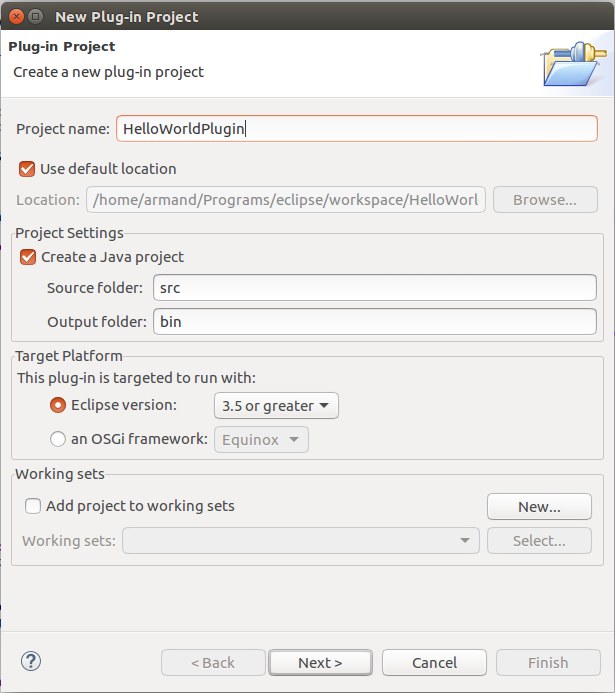
\includegraphics[width=0.4\linewidth]{pictures/newPlugin1.png}\label{fig:newPlugin1}}}%
    \qquad
\subfloat[Création d'un nouveau plugin - 2/4]{{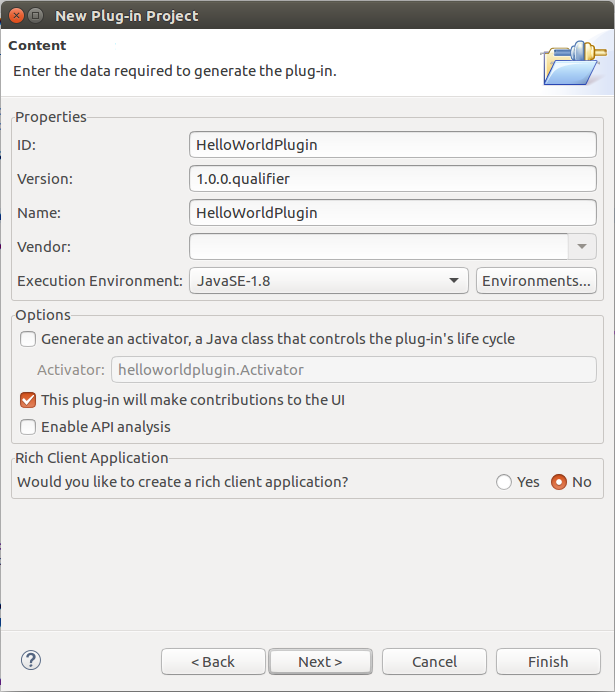
\includegraphics[width=0.4\linewidth]{pictures/newPlugin2.png}\label{fig:newPlugin2}}}%
    \vspace{0.5cm}
\centering
\subfloat[Création d'un nouveau plugin - 3/4]{{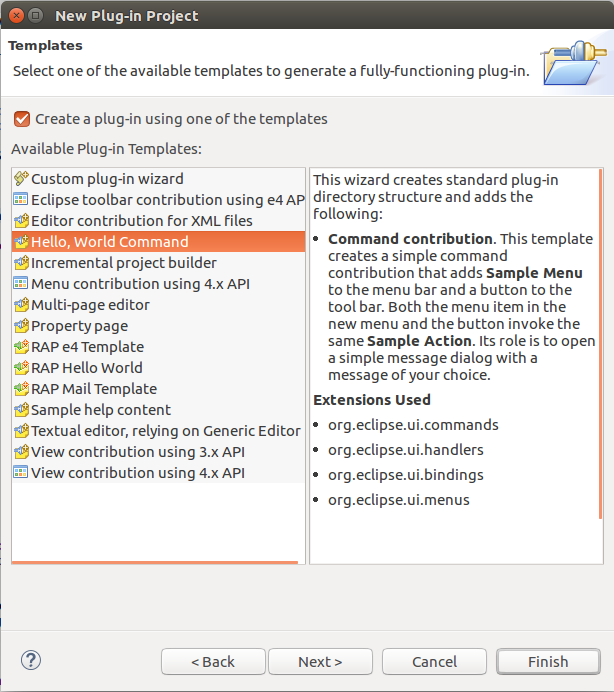
\includegraphics[width=0.4\linewidth]{pictures/newPlugin3.png}\label{fig:newPlugin3}}}%
    \qquad
\subfloat[Création d'un nouveau plugin - 4/4]{{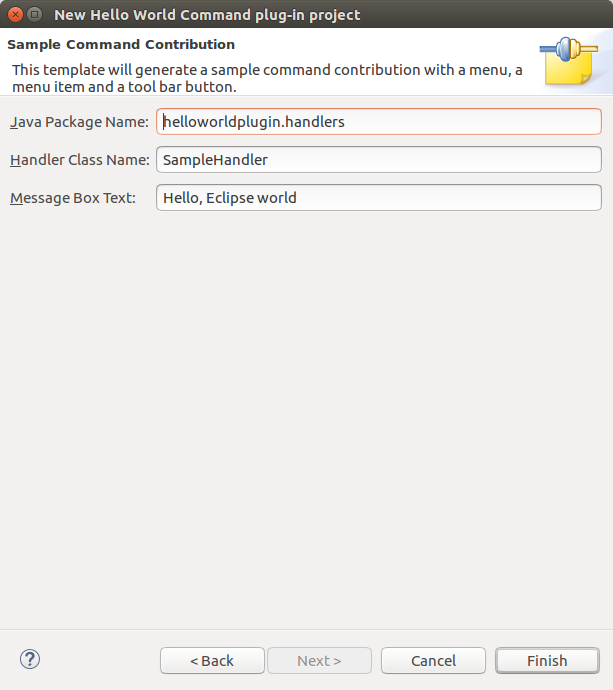
\includegraphics[width=0.4\linewidth]{pictures/newPlugin4.png}\label{fig:newPlugin4}}}%

\caption{Création d'un nouveau plugin dans Eclipse}
\end{figure}


La classe qui nous intéresse est \imtaInlinecode{java}{SampleHandler}, se trouvant dans \imtaInlinecode{text}{./src/helloworldplugin.handlers}.

\begin{imtaCode}{java}
public class SampleHandler extends AbstractHandler {

    @Override
    public Object execute(ExecutionEvent event) throws ExecutionException {
        IWorkbenchWindow window = HandlerUtil.getActiveWorkbenchWindowChecked(event);
            MessageDialog.openInformation(
                            window.getShell(),
                            "HelloWorldPlugin",
                            "Hello, Eclipse world");
            return null;
    }
}
\end{imtaCode}

Nous exécutons le plugin \textit{via} le menu \textit{Run > Run Configurations...}, où nous choisisson \textit{Eclipse Application}, sélectionnons \textit{org.eclipse.platform.ide} %
dans l'encadré \textit{Program to Run} sous l'option \textit{Run a product}.
Enfin, nous cliquons sur \textit{Run}.
Une nouvelle instance d'Eclipse s'ouvre, avec un bouton supplémentaire correspondant à notre plugin.
Lorsque nous cliquons sur celui-ci, une fenêtre s'ouvre, affichant le message \textit{"Hello, Eclipse world"}.

\subsection{Intégration dans Rodin}

\subsection{Appels à l'API de Rodin}
